\scanpage{16}
et par suite $\Sigma_2^-\cup\Sigma_{\deleted{\unsure{2}}1}^+$ \deleted{\unsure{sera|sont}} est un ouvert
% G03: word origin (1460,100); rule locus (1526,148)--(1669,158).
\begin{tikzpicture}[x=.012cm,y=-.012cm,baseline=(connexe.base)]
 \path[use as bounding box] (0,0) rectangle (213,65);
 \node[anchor=base west,inner sep=0pt,outer sep=0pt] (connexe) at (0,39) {connexe};
 \node[anchor=base west,inner sep=0pt,outer sep=0pt] at (66,51) {\unsure{\begin{tikzpicture}[x=.012cm,y=-.012cm,baseline=0pt]
  \path[use as bounding box] (0,-3) rectangle (143,8);
  \draw[line width=.35pt] (0,0) .. controls (43,-2) and (83,2) .. (143,6);
 \end{tikzpicture}}};
\end{tikzpicture}
de $X$ donc de $X\setminus E_2$, contenant
% G01: full-scan origin (1165,145); the inserted text and its guide occur once.
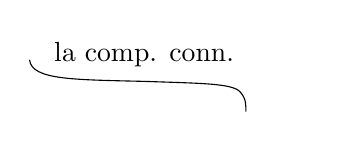
\begin{tikzpicture}[x=.012cm,y=-.012cm,baseline=(insone.base)]
 \path[use as bounding box] (0,0) rectangle (325,93);
 \node[anchor=base west,inner sep=0pt,outer sep=0pt] (insone) at (28,36) {\inserted{la comp. conn.}};
 \draw[line width=.4pt] (2,34) .. controls (4,56) and (51,55) .. (128,57)
  .. controls (184,59) and (217,59) .. (225,68)
  .. controls (232,76) and (231,83) .. (231,89);
\end{tikzpicture}
$\Sigma_2^-$
% G02: full-scan origin (1522,176); the comma below/left is represented by the following ordinary comma.
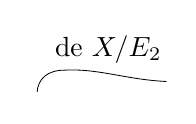
\begin{tikzpicture}[x=.012cm,y=-.012cm,baseline=(instwo.base)]
 \path[use as bounding box] (0,0) rectangle (148,72);
 \node[anchor=base west,inner sep=0pt,outer sep=0pt] (instwo) at (29,30) {\inserted{de $X/E_{\unsure{2}}$}};
 \draw[line width=.3pt] (10,68) .. controls (11,55) and (20,45) .. (39,45)
  .. controls (75,43) and (104,55) .. (147,57);
\end{tikzpicture}, donc \deleted{\unsure{c'est}} \unsure{é|ê}gal\unsure{e|} : $\Sigma_2^-$, donc $\Sigma_1^+\subset\Sigma_2^-$, \unsure{cqfd|qfd}

L'intersection des deux partitions
\[
 \begin{aligned}
 X&=\deleted{\unsure{E}}\Sigma_1^+\amalg E_1\amalg\Sigma_1^-\\
 X&=\Sigma_2^+\amalg E_2\amalg\Sigma_2^-
 \end{aligned}
\]
de $X$ est
% Central display: full-scan origin (500,800), .012cm per source pixel, y downward.
% G04 is the isolated point at (1139,842); its character, role, hand and surface origin remain open.
\figure{\begin{tikzpicture}[x=.012cm,y=-.012cm,baseline=0pt]
 \path[use as bounding box] (0,0) rectangle (1040,244);
 \node[anchor=base west,inner sep=0pt,outer sep=0pt] at (10,143) {$X=$};
 \node[anchor=base west,inner sep=0pt,outer sep=0pt] at (146,140) {$\Sigma_1^+$};
 \node[anchor=base west,inner sep=0pt,outer sep=0pt] at (260,140) {$\amalg$};
 \node[anchor=base west,inner sep=0pt,outer sep=0pt] at (339,140) {$E_1$};
 \node[anchor=base west,inner sep=0pt,outer sep=0pt] at (425,140) {$\amalg$};
 \node[anchor=base west,inner sep=0pt,outer sep=0pt] at (508,140) {$\deleted{E}\Sigma_{12}$};
 \node[anchor=base west,inner sep=0pt,outer sep=0pt] at (650,140) {$\amalg$};
 \node[anchor=base west,inner sep=0pt,outer sep=0pt] at (749,140) {$E_2$};
 \node[anchor=base west,inner sep=0pt,outer sep=0pt] at (843,140) {$\amalg$};
 \node[anchor=base west,inner sep=0pt,outer sep=0pt] at (923,140) {$\Sigma_2^+$};
 % BR01, observed upper brace: complete run and hooked right end.
 \draw[line width=.4pt] (161,78) .. controls (192,57) and (220,53) .. (261,63)
  .. controls (286,67) and (306,63) .. (317,49)
  .. controls (325,58) and (340,62) .. (361,62)
  .. controls (439,63) and (510,54) .. (547,54)
  .. controls (563,54) and (565,59) .. (563,65);
 \node[anchor=base west,inner sep=0pt,outer sep=0pt] at (332,44) {$\Sigma_2^-$};
 % BR02, observed lower brace: starts beneath the 12 area.
 \draw[line width=.4pt] (585,160) .. controls (602,179) and (638,181) .. (682,175)
  .. controls (720,171) and (747,170) .. (760,170)
  .. controls (765,170) and (764,177) .. (765,181)
  .. controls (772,171) and (791,171) .. (831,171)
  .. controls (884,171) and (923,174) .. (956,170)
  .. controls (961,170) and (962,167) .. (963,163);
 \node[anchor=base west,inner sep=0pt,outer sep=0pt] at (735,236) {$\Sigma_1^-$};
 \node[anchor=base west,inner sep=0pt,outer sep=0pt] at (637,39) {\unsure{\begin{tikzpicture}[x=.012cm,y=-.012cm,baseline=0pt]
  \path[use as bounding box] (0,0) rectangle (5,6);
  \fill[black!50] (1,1) .. controls (4,0) and (5,4) .. (3,5) .. controls (1,6) and (0,3) .. cycle;
 \end{tikzpicture}}};
\end{tikzpicture}}

% G05: the isolated point below/right of avec. Full-scan origin (257,1034).
\begin{tikzpicture}[x=.012cm,y=-.012cm,baseline=(avec.base)]
 \path[use as bounding box] (0,0) rectangle (237,126);
 \node[anchor=base west,inner sep=0pt,outer sep=0pt] (avec) at (14,47) {avec};
 \node[anchor=base west,inner sep=0pt,outer sep=0pt] at (171,92) {\unsure{\begin{tikzpicture}[x=.012cm,y=-.012cm,baseline=0pt]
  \path[use as bounding box] (0,0) rectangle (5,5);
  \fill (1,1) .. controls (4,0) and (5,3) .. (3,4) .. controls (1,5) and (0,3) .. cycle;
 \end{tikzpicture}}};
\end{tikzpicture}
\[
 \Sigma_{12}\overset{\text{def}}{=}\Sigma_1^-\cap\Sigma_2^-
\]

\deleted{\unsure{O}}Dans cette partition, $\Sigma_1^+,\Sigma_{12},\Sigma_2^+$ sont ouverts $E_1,E_2$ sont fermés, et on a
\[
 \begin{aligned}
 &\Sigma_1^+\subsetneq\overline{\Sigma_1^+}\subset\Sigma_1^+\cup E_1\\
 &\overline{\Sigma_{12}}\subset\overline{\Sigma_1^-}\cap\overline{\Sigma_2^-}\subset
 (\Sigma_1^-\cup E_1)\cap(\Sigma_2^-\cup E_2)\subset\Sigma_{12}\cup E_1\cup E_2\\
 &\Sigma_2^+\subsetneq\overline{\Sigma_2^+}\subset\Sigma_2^+\cup E_2
 \end{aligned}
\]
% G06: two detached points at the right margin, full-scan origin (1618,1726).
\margin{\unsure{\begin{tikzpicture}[x=.025cm,y=-.025cm,baseline=0pt]
 \path[use as bounding box] (0,0) rectangle (12,17);
 \fill (6,2) .. controls (9,0) and (10,4) .. (8,5) .. controls (5,6) and (4,4) .. cycle;
 \fill (1,10) .. controls (3,8) and (6,10) .. (5,13) .. controls (3,15) and (0,13) .. cycle;
\end{tikzpicture}}}

Notons aussi que
% G07: the detached point above the second formula; full-scan display origin (320,1890).
\figure{\begin{tikzpicture}[x=.012cm,y=-.012cm,baseline=0pt]
 \path[use as bounding box] (0,0) rectangle (810,116);
 \node[anchor=base west,inner sep=0pt,outer sep=0pt] at (10,103) {$\overline{\Sigma_{12}}\cap E_1\ne\varnothing,$};
 \node[anchor=base west,inner sep=0pt,outer sep=0pt] at (465,103) {$\overline{\Sigma_{12}}\cap E_2\ne\varnothing$};
 \node[anchor=base west,inner sep=0pt,outer sep=0pt] at (606,2) {\unsure{\begin{tikzpicture}[x=.012cm,y=-.012cm,baseline=0pt]
  \path[use as bounding box] (0,0) rectangle (5,6);
  \fill (1,1) .. controls (3,0) and (3,2) .. (4,4) .. controls (3,6) and (0,5) .. cycle;
 \end{tikzpicture}}};
\end{tikzpicture}}

Car si on avait p.\,ex. $\overline{\deleted{\unsure{E}}\Sigma_{12}}\cap
\deleted{\unsure{\Sigma}}E_1=\varnothing$, on
% G08: full-scan origin (286,2104); actual curved strike, no added generic visible strike.
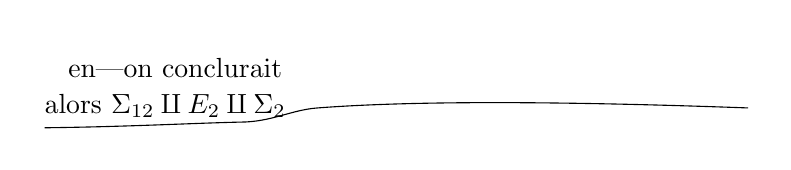
\begin{tikzpicture}[x=.012cm,y=-.012cm,baseline=(cancelled.base)]
 \path[use as bounding box] (0,0) rectangle (779,121);
 \node[anchor=base west,inner sep=0pt,outer sep=0pt] (cancelled) at (18,91)
  {\rlap{alors $\Sigma_{12}\amalg E_2\amalg\Sigma_2$}\phantom{\deleted{alors $\Sigma_{12}\amalg E_2\amalg\Sigma_2$}}};
 \node[anchor=base west,inner sep=0pt,outer sep=0pt] at (43,53) {\inserted{\unsure{en|on} conclurait}};
 \draw[line width=.4pt] (18,106) .. controls (104,105) and (179,101) .. (225,100)
  .. controls (258,100) and (279,87) .. (307,85)
  .. controls (412,77) and (570,78) .. (763,85);
\end{tikzpicture}
$\overline{\Sigma_1^-}\cap E_1=\varnothing$,
\[
 \begin{aligned}
 \big[\,\text{car}\quad\overline{\Sigma_1^-}&=
 \overline{\Sigma_2^+\deleted{\amalg}\unsure{\cup|\amalg} E_2
 \deleted{\amalg}\unsure{\cup|\amalg}\Sigma_{12}}=\,
 % G09: local origin (1090,2228), hooked/retraced underbrace and its label.
 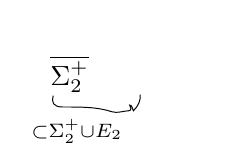
\begin{tikzpicture}[x=.012cm,y=-.012cm,baseline=(closed.base)]
  \path[use as bounding box] (20,0) rectangle (226,119);
  \node[anchor=base west,inner sep=0pt,outer sep=0pt] (closed) at (44,61) {$\overline{\Sigma_2^+}$};
  \draw[line width=.35pt] (47,72) .. controls (45,79) and (47,84) .. (57,84)
   .. controls (78,84) and (94,84) .. (109,89)
   .. controls (115,91) and (122,88) .. (127,88)
   .. controls (130,88) and (130,84) .. (128,82)
   .. controls (131,82) and (131,87) .. (132,88)
   .. controls (137,83) and (140,77) .. (139,71);
  \node[anchor=base west,inner sep=0pt,outer sep=0pt] at (24,116) {$\scriptstyle\subset\Sigma_2^+\cup E_2$};
 \end{tikzpicture}
 \cup E_2\cup\overline{\Sigma_{12}}\subset\Sigma_1^-\cup\overline{\Sigma_{12}}
 % G10: closing-bracket candidate; only observed returns, no supplied upright.
 \unsure{\begin{tikzpicture}[x=.012cm,y=-.012cm,baseline=0pt]
  % Full-scan origin (1630,2215); visible source bounds extend to x=1670.
  \path[use as bounding box] (0,0) rectangle (41,116);
  \draw[line width=.4pt] (11,3) -- (13,7)
   .. controls (24,7) and (34,8) .. (40,13);
  \draw[line width=.4pt] (0,111) .. controls (13,112) and (25,108) .. (40,111);
 \end{tikzpicture}}
 \end{aligned}
\]
ce qui n'est pas.

% archive sheet number: 15
